\selectlanguage{english}
\clearpage
\section{Theoretical Foundations}

In this chapter, the theoretical background necessary to understand the development of a system testing framework for eCAL is presented. Section 2.1 introduces essential concepts in software testing, such as test levels, types, and techniques. Section 2.2 explains the concept of distributed systems, including their characteristics and common use cases. Section 2.3 provides the fundamentals of inter-process communication (IPC) and highlights different communication mechanisms. In Section 2.4, the role of middleware in distributed environments is discussed, with a focus on commonly used solutions such as ROS, DDS, and eCAL. Finally, Section 2.5 outlines specific challenges in testing middleware systems, presents current testing approaches, and analyzes the limitations of testing practices in the context of eCAL.

\subsection{Software Testing Fundamentals}

Software testing is a structured process aimed at verifying that software meets the defined requirements and performs reliably in its intended environment. This section introduces the core concepts of software testing, including test levels, test types, test techniques, and the test pyramid.

\subsubsection{Test Levels}

Software testing is organized into different levels to detect defects at specific stages of development. According to Ammann and Offutt \cite{ammann2016introduction}, the main test levels are:

\vspace{1em}
\textbf{Unit Testing:}

\vspace{0.4em}
Unit testing focuses on verifying individual components or units of a system in isolation. These tests are typically written and executed by developers during the coding phase and aim to detect logic errors or incorrect function outputs early \cite{pressman2014software}, \cite{spillner2019softwaretest}.

\vspace{1em}
\textbf{Integration Testing:}

\vspace{0.4em}
Integration testing validates the interaction between different modules or components. This level ensures that data is correctly passed and interpreted between integrated parts of the application \cite{burnstein2003practical}, \cite{spillner2019softwaretest}.

\newpage

\textbf{System Testing:}

\vspace{0.4em}
System testing examines the entire integrated system as a whole. It verifies that the system behaves correctly under various conditions, including performance, security, and usability aspects \cite{myers2011art}, \cite{spillner2019softwaretest}.

\vspace{1em}
In distributed systems, however, the boundary between integration testing and system testing can become blurred. Since individual components often run on different machines or communicate asynchronously, validating their interaction frequently involves testing parts of the overall system behavior as well. As a result, what is formally considered integration testing may already include system-level characteristics such as network latency, synchronization, or fault tolerance.

\vspace{1em}
\textbf{Acceptance Testing:}

\vspace{0.4em}
Acceptance testing, also called User Acceptance Testing (UAT), determines whether the software fulfills the business requirements and is ready for deployment. It is usually performed by end users or stakeholders \cite{kaner1999testing}.
\vspace{0.2em}

\subsubsection{Test Types}

There are two major types of tests commonly used in software quality assurance:

\vspace{1em}
\textbf{A) Functional Testing}

\vspace{0.4em}
Functional testing ensures that software features behave according to their specifications. It is typically performed through techniques like equivalence class partitioning and boundary value analysis \cite{pressman2014software}.

\vspace{1em}
\textbf{B) Non-functional Testing}

\vspace{0.4em}
Non-functional testing addresses aspects such as performance, reliability, maintainability, and usability. These qualities are essential for a software product to function effectively in production environments \cite{kaner1999testing}.

\vspace{0.4em}
\subsubsection{Test Techniques}

Various techniques are used to design efficient and targeted test cases:

\vspace{1em}
\textbf{Black-Box Testing}

\vspace{0.4em}
Black-box testing validates the system's functionality without considering its internal code structure. Testers use input-output analysis to confirm expected behavior \cite{myers2011art}, \cite{spillner2019softwaretest}.

\vspace{1em}
\textbf{White-Box Testing}

\vspace{0.4em}
White-box testing is based on knowledge of the internal structure and logic of the system. Testers examine decision paths, loops, and control structures to ensure code coverage \cite{burnstein2003practical}, \cite{spillner2019softwaretest}.

\vspace{1em}
\textbf{Gray-Box Testing}

\vspace{0.4em}
Gray-box testing combines elements of black-box and white-box approaches. It requires partial knowledge of the internal workings to create more targeted and effective test cases \cite{ammann2016introduction}, \cite{spillner2019softwaretest}.

\subsubsection{Test Pyramid}

The test pyramid is a widely recognized concept used to structure testing strategies in a scalable and maintainable way. It was introduced by Mike Cohn \cite{cohn2009succeeding} to help development teams allocate their testing efforts effectively across different levels of abstraction.

\vspace{2em}
\begin{figure}[H]
	\centering
	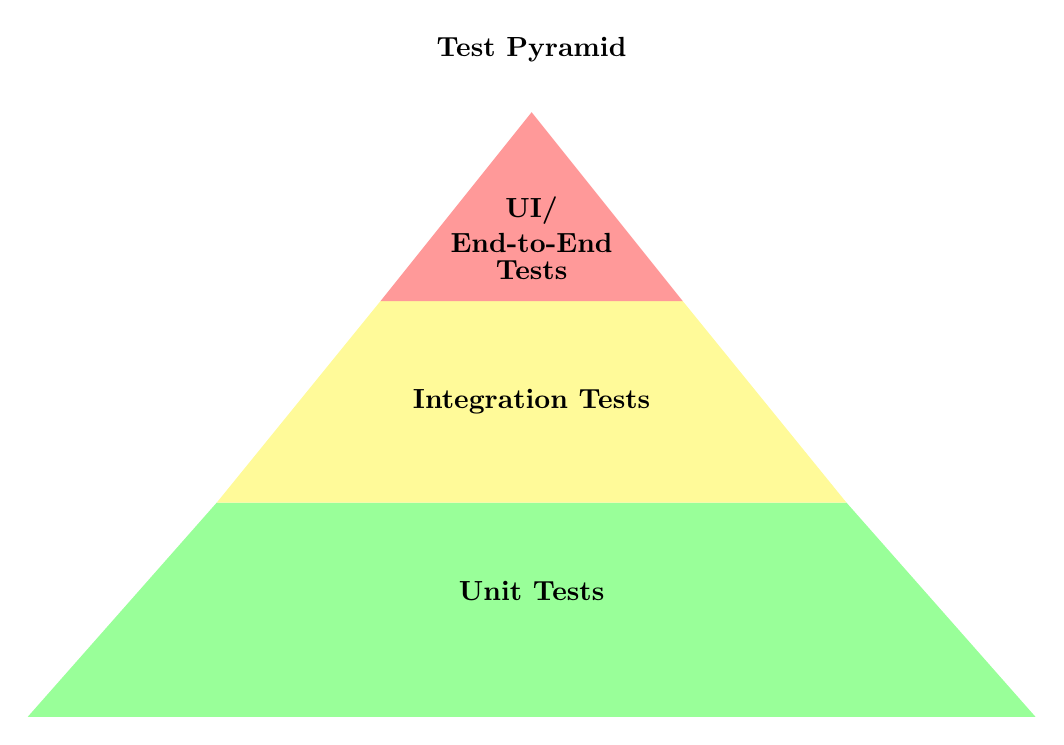
\begin{tikzpicture}[scale=1.6]
		
		% Bottom Layer: Unit Tests
		\fill[green!40] (0,0) -- (8,0) -- (6.5,1.7) -- (1.5,1.7) -- cycle;
		
		% Middle Layer: Integration Tests
		\fill[yellow!40] (1.5,1.7) -- (6.5,1.7) -- (5.2,3.3) -- (2.8,3.3) -- cycle;
		
		% Top Layer: UI Tests
		\fill[red!40] (2.8,3.3) -- (5.2,3.3) -- (4,4.8) -- cycle;
		
		
		% Labels
		\node at (4,1) {\textbf{Unit Tests}};
		\node at (4,2.5) {\textbf{Integration Tests}};
		\node at (4,3.8) {\shortstack{\textbf{UI/}\\\textbf{End-to-End}\\\textbf{Tests}}};
		
		% Title
		\node[font=\bfseries] at (4,5.3) {Test Pyramid};
		
	\end{tikzpicture}
	\caption{The Test Pyramid illustrating test distribution across levels (adapted from Cohn \cite{cohn2009succeeding}).}
	\label{fig:testpyramid}
\end{figure}

\newpage
At the base of the pyramid lies a large number of unit tests. These are fast, automated, and verify individual components or functions in isolation. Unit tests provide immediate feedback during development and help detect issues early, making them the foundation of efficient software testing.

\vspace{1em}
The middle layer consists of fewer integration tests. These tests check how different modules or components interact with each other and help uncover interface-related defects that are not visible during unit testing.

\vspace{1em}
At the top of the pyramid are the end-to-end or UI tests. These are high-level tests that simulate real user interactions across the entire system. Although essential for validating system behavior from a user perspective, they are typically slower, more fragile, and more expensive to maintain.

\vspace{1em}
As visualized in Figure~\ref{fig:testpyramid}, the pyramid illustrates the principle that lower-level tests should be more numerous and faster, while higher-level tests should be fewer and more focused. This structure promotes reliable, maintainable, and cost-effective testing workflows.

\subsection{Distributed Systems}

\subsubsection{Definition and Concepts}

A distributed system is a network of independent computers that appears to users as a single coherent system. In distributed systems, multiple computing devices communicate and coordinate their activities by passing messages to achieve a common goal \cite{tanenbaum2017}. Such systems consist of independent components located on different networked computers, which interact with each other by exchanging messages.

\vspace{1em}
The primary goal of distributed systems is to share resources, increase performance, and provide reliable and fault-tolerant operations. Resources such as processing power, memory, storage, and data can be shared between multiple nodes within the system, enhancing system efficiency and scalability \cite{coulouris2012}.

\vspace{1em}
Figure~\ref{fig:distributed_architecture} illustrates a basic distributed system consisting of multiple independent nodes communicating over a network. Each node may serve a specific role, such as providing services, accessing shared resources, or coordinating tasks.

\begin{figure}[H]
	\centering
	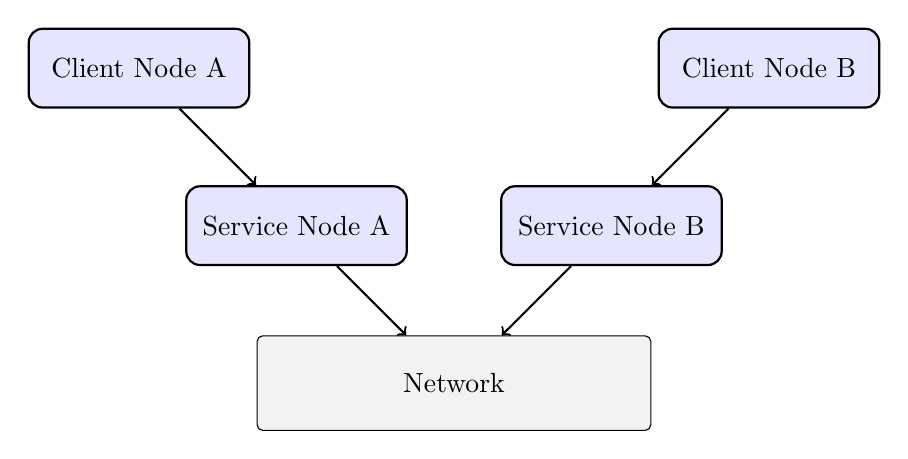
\begin{tikzpicture}[
		node/.style={draw, thick, minimum width=2.8cm, minimum height=1cm, rounded corners=5pt, fill=blue!10},
		conn/.style={->, thick},
		network/.style={draw, fill=gray!10, rounded corners=2pt}
		]
		
		% Nodes
		\node[node] (client1) at (-4, 2) {Client Node A};
		\node[node] (client2) at (4, 2) {Client Node B};
		\node[node] (server1) at (-2, 0) {Service Node A};
		\node[node] (server2) at (2, 0) {Service Node B};
		
		% Network Cloud
		\node[network, minimum width=5cm, minimum height=1.2cm] (network) at (0,-2) {Network};
		
		% Arrows from Clients to Services
		\draw[conn] (client1) -- (server1);
		\draw[conn] (client2) -- (server2);
		
		% Arrows from Services to Network
		\draw[conn] (server1) -- (network);
		\draw[conn] (server2) -- (network);
		
	\end{tikzpicture}
	\caption{Basic architecture of a distributed system with multiple clients and services connected through a network}
	\label{fig:distributed_architecture}
\end{figure}


\subsubsection{Characteristics and Challenges}

Distributed systems have several key characteristics, including concurrency, scalability, transparency, and fault tolerance. Concurrency refers to multiple processes executing simultaneously. Scalability describes the capability of the system to grow easily in size and workload. Transparency ensures the complexity of the system remains hidden from users, providing an impression of a single unified system. Fault tolerance describes the system's capability to continue operation even when individual components fail \cite{tanenbaum2017}.

\vspace{1em}
However, developing and managing distributed systems can be challenging. Problems related to communication delays, synchronization between processes, security, and managing the complexity of the overall system must be addressed effectively to ensure reliable operations \cite{coulouris2012}.

\subsubsection{Application Areas}

Distributed systems are widely used across many industries. In automotive systems, they support advanced driver-assistance systems (ADAS), autonomous driving, and vehicle communication systems. Robotics heavily relies on distributed systems for complex coordination tasks, such as collaborative robotics, autonomous navigation, and real-time control. The Internet of Things (IoT) is another prominent application area, where distributed systems enable efficient communication between countless smart devices and sensors, facilitating smart homes, smart cities, and industrial automation \cite{tanenbaum2017,coulouris2012}.



\subsection{Inter-Process Communication (IPC)}

\subsubsection{Overview and Importance}

Inter-process communication (IPC) refers to mechanisms that allow processes to communicate and exchange data. IPC is a crucial component in distributed and concurrent systems, enabling different software processes running on one or multiple computers to coordinate and share information effectively \cite{stallings2018}. Effective IPC mechanisms are essential for ensuring the smooth and reliable functioning of complex software systems, especially in critical applications such as automotive control systems, robotics, and industrial automation \cite{tanenbaum2015}.

\subsubsection{Common IPC Mechanisms}

There are several commonly used IPC mechanisms, each suitable for different scenarios and requirements. The most frequently used methods include shared memory, message passing, and remote procedure calls \cite{stallings2018,tanenbaum2015}.

\vspace{1em}
\begin{figure}[H]
	\centering
	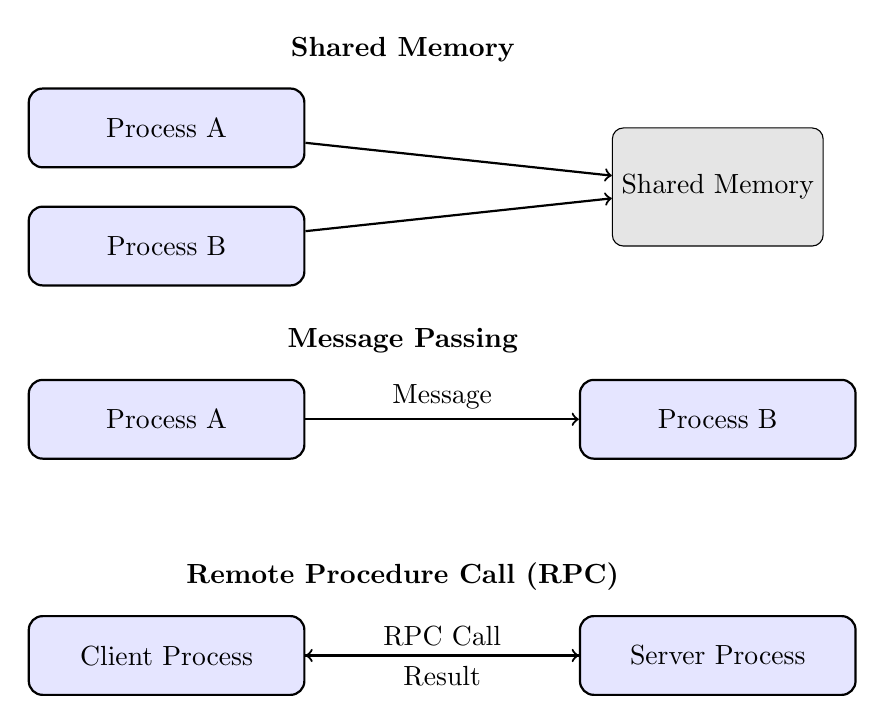
\begin{tikzpicture}[
		node/.style={draw, thick, minimum width=3.5cm, minimum height=1cm, rounded corners=5pt, fill=blue!10},
		conn/.style={->, thick},
		label/.style={font=\bfseries, align=center}
		]
		
		% Shared Memory
		\node[label] at (0,8) {Shared Memory};
		\node[node] (shmA) at (-3,7) {Process A};
		\node[node] (shmB) at (-3,5.5) {Process B};
		\node[draw, fill=gray!20, minimum width=2.5cm, minimum height=1.5cm, rounded corners=4pt] at (4,6.25) (shm) {Shared Memory};
		\draw[conn] (shmA) -- (shm);
		\draw[conn] (shmB) -- (shm);
		
		% Message Passing
		\node[label] at (0,4.3) {Message Passing};
		\node[node] (msgA) at (-3,3.3) {Process A};
		\node[node] (msgB) at (4,3.3) {Process B};
		\draw[conn] (msgA) -- node[above] {Message} (msgB);
		
		% RPC
		\node[label] at (0,1.3) {Remote Procedure Call (RPC)};
		\node[node] (rpcClient) at (-3,0.3) {Client Process};
		\node[node] (rpcServer) at (4,0.3) {Server Process};
		\draw[conn] (rpcClient) -- node[above] {RPC Call} (rpcServer);
		\draw[conn] (rpcServer) -- node[below] {Result} (rpcClient);
		
	\end{tikzpicture}
	\caption{Comparison of common IPC mechanisms: Shared Memory, Message Passing, and Remote Procedure Call (RPC)}
	\label{fig:ipc_methods}
\end{figure}


\vspace{1em}
\newpage
Figure~\ref{fig:ipc_methods} illustrates a simplified comparison of common IPC mechanisms. Shared memory allows processes to access a common memory region directly. Message passing transfers data through explicit send/receive actions. RPC abstracts communication by allowing a process to call functions in another process as if they were local.

\vspace{1em}
\textbf{Shared Memory:}

Shared memory is one of the fastest IPC methods, allowing processes to communicate directly by accessing a common area of memory. Processes write and read data directly into this shared space, avoiding the overhead of explicit communication. However, managing synchronization and ensuring data integrity can become challenging and requires careful implementation of synchronization methods, such as semaphores or mutexes \cite{stallings2018, ipc_performance_analysis}.

\vspace{1em}
\textbf{Message Passing:}

\vspace{0.4em}
Message passing involves processes communicating through messages. This approach ensures a clear separation between processes, providing safer communication. Messages are sent explicitly from one process to another using defined communication channels, such as pipes or sockets. While message passing typically has higher overhead compared to shared memory, it is easier to manage synchronization, and it allows better scalability in distributed environments \cite{tanenbaum2015}.

\vspace{1em}
\textbf{Remote Procedure Calls (RPC):}

\vspace{0.4em}
Remote Procedure Calls enable processes to invoke procedures or functions on remote systems as if they were local calls. RPC abstracts network communication, making distributed system interactions easier to develop and maintain. RPC is widely used in distributed applications and middleware solutions due to its simplicity and clear programming model, despite some performance overhead from serialization and network transmission \cite{coulouris2012}.

\subsubsection{Zero-Copy Communication}

Zero-copy communication is an advanced IPC technique designed to minimize unnecessary data copying between processes. Traditional communication methods often involve copying data multiple times, significantly reducing performance and increasing latency. Zero-copy mechanisms avoid this overhead by allowing direct data transfers between processes, usually through shared memory. By reducing the data copies, zero-copy enhances performance and efficiency in systems with high throughput and low latency requirements, such as high-performance computing or real-time systems \cite{raiciu2017}.



\subsection{Middleware in Distributed Systems}

While IPC mechanisms define how processes communicate, middleware abstract these and provide a structured interface for distributed applications.

\subsubsection{Definition and Role of Middleware}

Middleware is software that sits between applications and the underlying operating system or network infrastructure, enabling easier communication and coordination within distributed systems. Its main role is to simplify development by abstracting complexities associated with networked and distributed computing, such as communication protocols, data exchange, and interoperability between diverse systems \cite{bernstein1996}. Middleware allows software developers to focus more on the application logic rather than the low-level communication and network details.

\subsubsection{Common Middleware Solutions}

Various middleware technologies are available today, each designed to address specific communication and coordination needs. Some widely used middleware solutions include the Robot Operating System (ROS) \cite{quigley2009}, the Data Distribution Service (DDS) \cite{pardo2003}, and the enhanced Communication Abstraction Layer (eCAL) \cite{ecal_official_docs}.

\vspace{1em}
Table~\ref{tab:middleware_comparison} presents a layered architecture comparison between ROS, DDS, and eCAL. Each middleware abstracts the communication stack differently, but all provide core functionality for distributed system communication.

\begin{table}[H]
	\centering
	\renewcommand{\arraystretch}{1.20}
	\begin{tabular}{|p{2.25cm}|p{3.22cm}|p{3.22cm}|p{3.22cm}|}
		\hline
		\textbf{Layer} & \textbf{ROS} & \textbf{DDS} & \textbf{eCAL} \\
		\hline
		Application Layer & User Applications & User Applications & User Applications \\
		\hline
		Middleware API & rospy, roscpp & DDS API & eCAL API (C++, Python, etc.) \\
		\hline
		Core-Components & ROS-Master, Topics, Services & RTPS Protocol & Pub/Sub, RPC \\
		\hline
		Transport Layer & TCP-ROS, UDP-ROS & UDP/IP & Shared-Memory, UDP, TCP \\
		\hline
		Operating System & Linux, Windows, macOS & OS-dependent & Linux, Windows, macOS \\
		\hline
	\end{tabular}
	\caption{Architecture comparison between ROS, DDS, and eCAL middleware}
	\label{tab:middleware_comparison}
\end{table}

\vspace{1em}
\textbf{Robot Operating System (ROS):}
\vspace{0.4em}

ROS is an open-source middleware widely used in robotics. It provides a structured communication framework that includes services like message passing, data visualization, hardware abstraction, and numerous tools for robotics development. ROS simplifies building complex robotic systems by offering standardized communication interfaces and extensive community-supported tools and libraries \cite{quigley2009}.

\vspace{1em}
\textbf{Data Distribution Service (DDS):}
\vspace{0.4em}

DDS is a standardized middleware designed primarily for real-time and high-performance distributed applications. It employs a publisher-subscriber communication model, where components communicate by exchanging messages without direct connections between producers and consumers. DDS provides reliable and scalable communication, making it suitable for critical applications such as automotive systems, aerospace, industrial automation, and healthcare \cite{pardo2003}.

\vspace{1em}
\textbf{Enhanced Communication Abstraction Layer (eCAL):}
\vspace{0.4em}

The enhanced Communication Abstraction Layer (eCAL) is an open-source middleware designed specifically for efficient inter-process communication (IPC) in distributed environments. It simplifies the exchange of data between processes running on the same device or across multiple networked computers. eCAL uses a decentralized publish-subscribe architecture, allowing multiple processes to communicate directly without relying on a central broker \cite{ecal_github}.

\subsection{Testing in Middleware}

\subsubsection{Specific Challenges}

Testing middleware within distributed systems presents several challenges due to the complexity of distributed architectures and the abstract nature of middleware functionality. Middleware often operates across heterogeneous platforms and coordinates communication between independent software components. As Tanenbaum and van Steen emphasize, ensuring interoperability and consistent behavior across diverse systems introduces technical and architectural complexity \cite{tanenbaum2017}.

\newpage
A core challenge is compatibility, as middleware must support various hardware, operating systems, network protocols, and data formats. According to Coulouris, this requires middleware to provide standard abstractions while hiding platform-specific details \cite{coulouris2012}. 

\vspace{1em}
Performance and scalability also represent key testing concerns. Middleware must support low-latency communication and efficient resource use under variable loads. Stallings notes that poor synchronization or inefficient resource management at the middleware layer can lead to system-wide bottlenecks \cite{stallings2018}.

\vspace{1em}
Finally, fault tolerance and security must be evaluated, particularly since middleware can be a single point of failure or a vector for attack in distributed architectures \cite{liu2009middleware}.

\subsubsection{Existing Approaches and Best Practices}

Testing middleware systems effectively requires an understanding of the system architecture and the communication patterns it supports. Burns and Wellings suggest that model-based testing is particularly suited for middleware due to its ability to describe behavior across abstraction layers \cite{burns2009real}.

\vspace{1em}
{Integration testing plays a vital role in evaluating message routing, service discovery, and state synchronization among components. Additionally, system-level testing validates functional correctness and non-functional requirements, such as real-time constraints and message reliability \cite{gorton2006software}.

\vspace{1em}
Best practices include the use of simulation environments for performance evaluation under controlled conditions, as well as leveraging monitoring and logging tools to capture middleware-level interactions for post-test analysis. Gorton and Liu also highlight the use of profiling and benchmarking frameworks to test middleware scalability across node clusters \cite{gorton2006software}.

\vspace{1em}
In addition, techniques such as fault injection or failure simulation are particularly valuable when testing distributed middleware. These methods deliberately introduce faults such as: process termination, artificial network loss, or resource exhaustion. These observe how the system responds under edge cases. For containerized systems, this can be achieved through controlled Docker container crashes or simulated network partitions. Such tests are essential to verify the middleware's robustness and fault tolerance under realistic failure scenarios.
